\documentclass[aspectratio=169]{beamer}

\usepackage{tikz}
\usetikzlibrary{shapes, backgrounds, arrows, positioning}
\usepackage{listings}
\usepackage[utf8,latin1]{inputenc}
\usepackage[style = apa, backend = biber, natbib = true]{biblatex}
\addbibresource{../../literature/lit.bib}

\makeatletter \def\newblock{\beamer@newblock} \makeatother  

\beamertemplatenavigationsymbolsempty
\setbeamertemplate{itemize items}[circle]
\setbeamertemplate{section in toc}[circle]
\mode<beamer>{\setbeamercolor{math text displayed}{fg=iwmgray}}
\setbeamercolor{block body}{bg=iwmorange!50!white}
\setbeamercolor{block title}{fg=white, bg=iwmorange}

% Definitions for biblatex
\setbeamercolor{bibliography entry note}{fg=iwmgray}
\setbeamercolor{bibliography entry author}{fg=iwmgray}
\setbeamertemplate{bibliography item}{}

\definecolor{iwmorange}{RGB}{255,105,0}
\definecolor{iwmgray}{RGB}{67,79,79}
\definecolor{iwmblue}{RGB}{60,180,220}
\definecolor{iwmgreen}{RGB}{145,200,110}
\definecolor{iwmpurple}{RGB}{120,0,75}

\setbeamercolor{title}{fg=iwmorange}
\setbeamercolor{frametitle}{fg=iwmorange}
\setbeamercolor{structure}{fg=iwmorange}
\setbeamercolor{normal text}{fg=iwmgray}
\setbeamercolor{author}{fg=iwmgray}
\setbeamercolor{date}{fg=iwmgray}

\title{Repeated measures}
\author{Nora Wickelmaier}
\date{Last modified: \today}

\newcommand{\vect}[1]{\mathbf{#1}}
\newcommand{\mat}[1]{\mathbf{#1}}
\newcommand{\gvect}[1]{\boldsymbol{#1}}
\newcommand{\gmat}[1]{\boldsymbol{#1}}

\lstset{language = R,%
  basicstyle = \ttfamily\color{iwmgray},
  frame = single,
  rulecolor = \color{iwmgray},
  commentstyle = \slshape\color{iwmgreen},
  keywordstyle = \bfseries\color{iwmgray},
  identifierstyle = \color{iwmpurple},
  stringstyle = \color{iwmblue},
  numbers = none,%left,numberstyle = \tiny,
  basewidth = {.5em, .4em},
  showstringspaces = false,
  emphstyle = \color{red!50!white}}

\AtBeginSection[]{
  \frame{
    \tableofcontents[sectionstyle=show/hide, subsectionstyle=show/show/hide]}}

\setbeamertemplate{headline}{
 \begin{beamercolorbox}{section in head}
   \vskip5pt\insertsectionnavigationhorizontal{\paperwidth}{}{}\vskip2pt
 \end{beamercolorbox}
}

\setbeamertemplate{footline}{\vskip-2pt\hfill\insertframenumber$\;$\vskip2pt}

\begin{document}

\begin{frame}{}
\thispagestyle{empty}
\titlepage
\end{frame}

\begin{frame}{Outline}
\tableofcontents
\end{frame}

\section{Repeated measures ANOVA}

\begin{frame}{Model with one repeated measurement factor}
  \begin{itemize}
    \item When subjects are observed for more than two time points, we can
      model these data using a repeated measures ANOVA
    \item Data layout
\[ \begin{array}{c|cccccc}
              & \multicolumn{6}{c}{\text{Time point}} \\
\text{Subject} & 1 & 2 & \cdots & j & \cdots & n \\ \hline
1      & y_{11} & y_{12} & \cdots & y_{1j} & \cdots & y_{1n} \\
2      & y_{21} & y_{22} & \cdots & y_{2j} & \cdots & y_{2n} \\
\vdots & \vdots &        &        &        &        & \vdots \\
i      & y_{i1} & y_{i2} & \cdots & y_{ij} & \cdots & y_{in} \\
\vdots & \vdots &        &        &        &        & \vdots \\
N      & y_{N1} & y_{N2} & \cdots & y_{Nj} & \cdots & y_{Nn} \\
\end{array} \]
  \end{itemize}
\end{frame}


\begin{frame}{Statistical model}
  \begin{itemize}
    \item When we observe $i = 1, \ldots, N$ subjects for $j = 1, \ldots,
      n$ time points, we get
\[
  y_{ij} = \mu_0 + \tau_j + \upsilon_i + \varepsilon_{ij}
\]
with 

\begin{tabular}{ll}
  $\mu_0$ & grand mean\\
  $\tau_j$ & effect of time point $j$ equal for all subjects\\
  $\upsilon_i$ & effect of subject $i$ constant over time\\
  $\varepsilon_{ij}$ & error term for subject $i$ at time point $j$
\end{tabular}

\item Assumptions
\begin{itemize}
\item $\upsilon_i \sim N(0, \sigma^2_\upsilon)$ i.i.d.,
  $\sigma^2_\upsilon$ being the variance between subjects
\item $\varepsilon_{ij} \sim N(0, \sigma^2)$ i.i.d., $\sigma^2$ being
      the variance within subjects
    \item $\upsilon_i$ and $\varepsilon_{ij}$ are independent
\end{itemize}
  \end{itemize}
\end{frame}

\begin{frame}{Statistical model}
  \[
  y_{ij} = \mu_0 + \tau_j + \upsilon_i + \varepsilon_{ij}
  \]
\centering
  \begin{tabular}{ccccc}
    \hline
    response & grand mean & time effect & subject effect  & residual \\
    \hline
    $y_{11}$ & $\mu_0$ & $\tau_1$  & $\upsilon_{1}$ & $\varepsilon_{11}$ \\
    $y_{12}$ & $\mu_0$ & $\tau_2$  & $\upsilon_{1}$ & $\varepsilon_{12}$ \\
    $y_{13}$ & $\mu_0$ & $\tau_3$  & $\upsilon_{1}$ & $\varepsilon_{13}$ \\
    \vdots & \vdots & \vdots   &  \vdots & \vdots \\
    $y_{21}$ & $\mu_0$ & $\tau_1$  & $\upsilon_{2}$ & $\varepsilon_{21}$ \\
    $y_{22}$ & $\mu_0$ & $\tau_2$  & $\upsilon_{2}$ & $\varepsilon_{22}$ \\
    $y_{23}$ & $\mu_0$ & $\tau_3$  & $\upsilon_{2}$ & $\varepsilon_{23}$ \\
    \vdots & \vdots & \vdots   &  \vdots & \vdots \\
    $y_{Nn}$ & $\mu_0$ & $\tau_n$  & $\upsilon_{N}$ & $\varepsilon_{Nn}$ \\
    \hline\\[-2ex]
    \only<2>{$\sigma_{\upsilon}^2 + \sigma^2$ & & &
    $\sigma_{\upsilon}^2$ & $\sigma^2$} \\
  \end{tabular}
\end{frame}

\begin{frame}{Model properties}
  \begin{itemize}
    \item For the model, we have
\begin{align*}
  E(y_{ij})   &= \mu_0 + \tau_j \\
  Var(y_{ij}) &= Var(\mu_0 + \upsilon_i + \tau_j + \varepsilon_{ij})
               = \sigma^2_\upsilon + \sigma^2 \\
  Cov(y_{ij}, y_{i'j}) &= 0 \text{ for subjects } i \neq i' \\
  Cov(y_{ij}, y_{ij'}) &= \sigma^2_\upsilon \text{ for observations }
                          j \neq j'
\end{align*}
      \vspace{-.6cm}
\item The correlation between observations and subjects is
\[
  Corr(y_{ij}, y_{ij'}) = \frac{\sigma^2_\upsilon}{\sigma^2_\upsilon +
    \sigma^2}
\]
known as intraclass correlation (ICC)
  \end{itemize}
\end{frame}

\begin{frame}{Compound Symmetry}
  \begin{itemize}
    \item For the covariance matrix of the observations for
      one subject we get the so-called compound symmetry structure
\[
  \gvect{\Sigma}_{\vect{y}_i} = \sigma^2_\upsilon \vect{1} \vect{1}'
    + \sigma^2 \mat{I}
  = 
  \begin{pmatrix}
    \sigma^2_\upsilon + \sigma^2 & \sigma^2_\upsilon & \sigma^2_\upsilon &
      \cdots & \sigma^2_\upsilon \\
    \sigma^2_\upsilon & \sigma^2_\upsilon  + \sigma^2 & \sigma^2_\upsilon &
      \cdots & \sigma^2_\upsilon \\
    \vdots & & \ddots & & \vdots \\
    \sigma^2_\upsilon & \sigma^2_\upsilon  & \sigma^2_\upsilon &
      \cdots & \sigma^2_\upsilon + \sigma^2 \\
  \end{pmatrix}
\]
% \item The covariance matrix for all observations is consequently block diagonal
% \[
%   Cov(\vect{y}) =
%   \begin{pmatrix}
%   \gvect{\Sigma}_{\vect{y}_1} & 0 & 0 & \cdots & 0 \\
%   0  & \gvect{\Sigma}_{\vect{y}_2} & 0 & \cdots & 0 \\
%   \vdots &  & \ddots &  & \vdots \\
%   0 & 0 & 0 & \cdots & \gvect{\Sigma}_{\vect{y}_N} \\
%   \end{pmatrix}
% \]
% and, therefore, $Cov(\vect{y}) = \sigma^2 \mat{I}$ does not apply as in the
%   regular linear model
    \item The assumption of a compound symmetry structure is usually
      unrealistic for longitudinal data
    \item In general, successive observations are more strongly correlated
      than observations being farther apart (covariance is not constant)
    \item Variance increases with time, e.\,g., when some subjects are more
      responsive to a certain treatment than others
  \end{itemize}
\end{frame}

\section[Example]{Example: Depression and Imipramin}

\begin{frame}{Depression and Imipramin \citep{ReisbyGram77}}
  \begin{itemize}
    \item \citet{ReisbyGram77} studied the effect of Imipramin on 66
      inpatients treated for depression
    \item Depression was measured with the Hamilton depression rating scale
      (HDRS)
    \item Additionally, the concentration of Imipramin and its metabolite
      Desipramin was measured in their blood plasma
    \item Patients were classified into endogenous and non-endogenous
      depressed
    \item Depression was measured weekly for 6 time points; the effect of
      the antidepressant was observed starting at week 2 for four weeks
  \end{itemize}
\end{frame}




\begin{frame}{Descriptive statistics}
\begin{columns}
\begin{column}{.55\textwidth}
  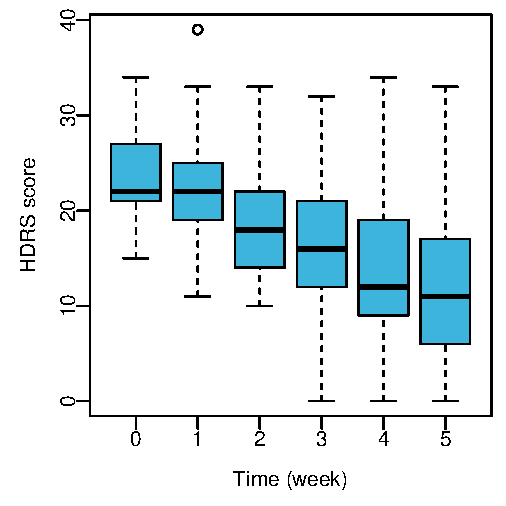
\includegraphics[scale=.8]{../figures/hdrs-box}
\end{column}
\begin{column}{.6\textwidth}
  HDRS score\\[1ex]
  {\footnotesize
\begin{tabular}{rrrrrrr}
  \hline
  $t$ & W0 & W1 & W2 & W3 & W4 & W5 \\ 
  \hline
  $M$  & 23.44 & 21.84 & 18.31 & 16.42 & 13.62 & 11.95 \\ 
  $SD$ &  4.53 & 4.70  & 5.49  & 6.42  & 6.97  & 7.22 \\ 
  $n$  & 61    & 63    & 65    & 65    & 63    & 58    \\ 
  \hline
\end{tabular}
  }

  \vspace{.5cm}
  Empirical correlation matrix of HDRS score\\[1ex]
  {\footnotesize
\begin{tabular}{rrrrrrr}
  \hline
   & W0 & W1 & W2 & W3 & W4 & W5 \\ 
  \hline
  Week 0 &   1 & .49 & .41 & .33 & .23 & .18 \\ 
  Week 1 & .49 &   1 & .49 & .41 & .31 & .22 \\ 
  Week 2 & .41 & .49 &   1 & .74 & .67 & .46 \\ 
  Week 3 & .33 & .41 & .74 &   1 & .82 & .57 \\ 
  Week 4 & .23 & .31 & .67 & .82 &   1 & .65 \\ 
  Week 5 & .18 & .22 & .46 & .57 & .65 &   1 \\ 
  \hline
\end{tabular}
  }

  \vspace{1cm}
\end{column}
\end{columns}
\end{frame}

\begin{frame}[fragile]{Depression and Imipramin}
  \begin{lstlisting}
dat      <- read.table("data/reisby.dat", header = TRUE)
dat$id   <- factor(dat$id)
dat$diag <- factor(dat$diag, levels = c("nonen", "endog"))
dat      <- na.omit(dat)     # drop missing values

# descriptive statistics
aggregate(hamd ~ week, dat, mean)
aggregate(hamd ~ week, dat, sd)
aggregate(hamd ~ week, dat, length)
dat[, c("hamd", "id", "week")] |>
  reshape(direction = "wide", timevar = "week") |>
  dplyr::select(-id) |>
  cor(use = "pairwise.complete.obs") |>
  round(3)
  \end{lstlisting}
\end{frame}

\begin{frame}[fragile]{Fitting repeated-measures ANOVA}
  \begin{lstlisting}
# week needs to be a factor when computing an ANOVA
dat$week2 <- factor(dat$week)
contrasts(dat$week2) <- "contr.sum"   # effect coding
summary(aov(hamd ~ week2 + Error(id + id:week2), dat))
# --> ??

library(ez)   # "SPSS"-style
ezANOVA(data = dat, dv = hamd, wid = id, within = week2, type = 3)

# check data
ezDesign(data = dat, x = week2, y = id, col = diag)
replications(hamd ~ week2 + id, dat)
  \end{lstlisting}
\end{frame}

\begin{frame}[fragile]{Fitting repeated-measures ANOVA}
  \begin{lstlisting}
# remove IDs with missing observations
ids <- names(which(replications(hamd ~ id, dat)$id == 6))
dat_val <- dat[dat$id %in% ids, ]

# fit ANOVAs again
aov1 <- aov(hamd ~ week2 + Error(id/week2), dat_val)
summary(aov1)

ez1 <- ezANOVA(data = dat_val, dv = hamd, wid = id, within = week2)
ez1$ANOVA
  \end{lstlisting}
\end{frame}

\begin{frame}[fragile]{Fitting repeated-measures ANOVA}
  \begin{lstlisting}
# How close can we get with a mixed-effects model?
library(lme4)

lme1 <- lmer(hamd ~ week2 + (1 | id), dat_val)
anova(lme1)

# calculate mean sum of squares for id by hand
sp <- attr(VarCorr(lme1)$id, "stddev")
se <- sigma(lme1)
se^2 + 6 * sp^2
  \end{lstlisting}
\end{frame}

\section{Mixed-effects regression}

\begin{frame}{Depression and Imipramin -- individual processes}
  \vspace{-.2cm}
  \begin{center}
    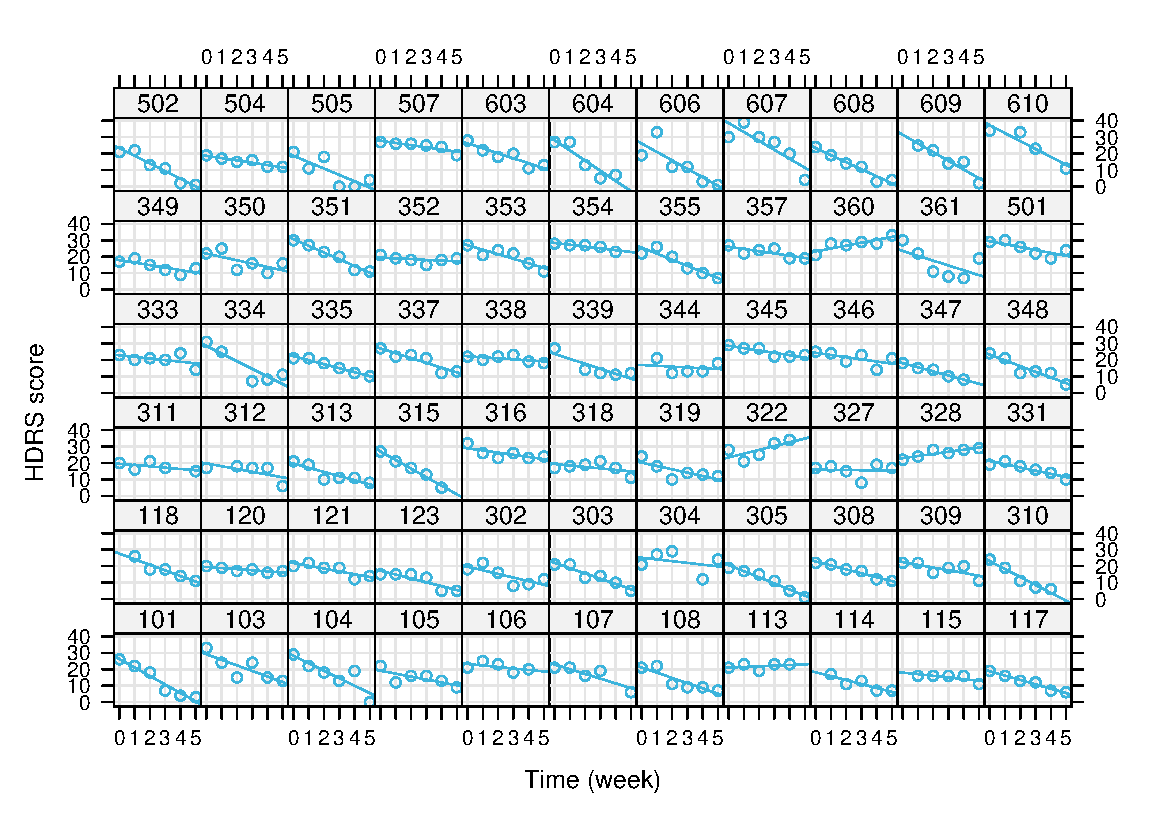
\includegraphics[width = 11cm]{../figures/hdrs-ind}
  \end{center}
\end{frame}

\begin{frame}{Alternative model with a constant time term}
  \centering
  \vspace{-1cm}
  \[
    y_{ij} = \beta_0 + \beta_1 time + \upsilon_{0i} + \varepsilon_{ij}
  \]
with $\upsilon_{0i} \sim N(0, \sigma^2_{\upsilon})$ i.i.d.,
$\varepsilon_{ij} \sim N(0, \sigma^2)$ i.i.d., $\upsilon_{0i}$ and
$\varepsilon_{ij}$ i.i.d.\\[2ex]
%  with $\varepsilon_{ij} \sim N(0, \sigma_{\varepsilon}^2)$ i.i.d.\ and
%  $\upsilon_{0i} \sim N(0, \sigma_{\upsilon})$ i.i.d.\\~\\

  \begin{tabular}{cccccc}
    \hline
    response & intercept & time effect & time & subject effect  & residual \\
    \hline
    $y_{11}$ & $\beta_0$ & $\beta_1$   & 0    & $\upsilon_{1}$ & $\varepsilon_{11}$ \\
    $y_{12}$ & $\beta_0$ & $\beta_1$   & 1    & $\upsilon_{1}$ & $\varepsilon_{12}$ \\
    $y_{13}$ & $\beta_0$ & $\beta_1$   & 2    & $\upsilon_{1}$ & $\varepsilon_{13}$ \\
    \vdots & \vdots & \vdots   & \vdots & \vdots & \vdots \\
    $y_{21}$ & $\beta_0$ & $\beta_1$   & 0    & $\upsilon_{2}$ & $\varepsilon_{21}$ \\
    $y_{22}$ & $\beta_0$ & $\beta_1$   & 1    & $\upsilon_{2}$ & $\varepsilon_{22}$ \\
    $y_{23}$ & $\beta_0$ & $\beta_1$   & 2    & $\upsilon_{2}$ & $\varepsilon_{23}$ \\
    \vdots & \vdots & \vdots   & \vdots & \vdots & \vdots \\
    $y_{Nn}$ & $\beta_0$ & $\beta_1$   & n    & $\upsilon_{N}$ & $\varepsilon_{Nn}$ \\
    \hline
  \end{tabular}
\end{frame}

\begin{frame}[fragile]{Random intercept model}
  \[
    y_{ij} = \beta_0 + \beta_1 time + \upsilon_{0i} + \varepsilon_{ij}
  \]
with $\upsilon_{0i} \sim N(0, \sigma^2_{\upsilon})$ i.i.d.,
$\varepsilon_{ij} \sim N(0, \sigma^2)$ i.i.d., $\upsilon_{0i}$ and
$\varepsilon_{ij}$ i.i.d.\\[2ex]
\begin{columns}
\begin{column}{.4\textwidth}
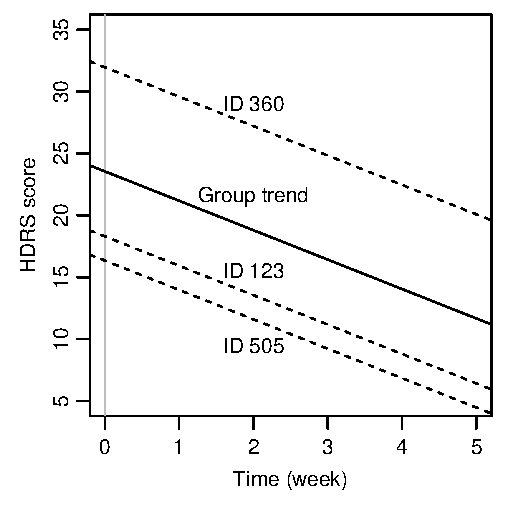
\includegraphics[width=5.5cm]{../figures/hdrs-lme1}
\end{column}
%
\begin{column}{.5\textwidth}
  \begin{itemize}
    \item The estimated mean baseline HDRS score is $\hat{\beta}_0 =
      23.55$
    \item However, the estimated standard deviation between patients is
      $\hat{\sigma}_\upsilon = 4.02$
    \item The mean improvement per week is $\hat{\beta}_1 = -2.38$
  \end{itemize}
  \vspace{1cm}
\end{column}
\end{columns}
\end{frame}

\begin{frame}{Implied marginal covariance matrix}
  \begin{itemize}
    \item For the three time points $t_{ij} = 0, 1, 2$, $\mat{Z}_i =
      \vect{1}'_{n_i}$ and $\gmat{\Sigma}_\upsilon = \sigma^2_\upsilon$ we
      get
\begin{align*}
  Cov(\vect{y}_i) &=
    \mat{Z}_i \gmat{\Sigma}_\upsilon \mat{Z}'_i + \sigma^2 \mat{I}_{n_i} \\
  &= \sigma^2_\upsilon \vect{1}_{n_i} \vect{1}'_{n_i} +
     \sigma^2 \mat{I}_{n_i} \\
  &= 
  \begin{pmatrix}
    \sigma^2_\upsilon + \sigma^2 & \sigma^2_\upsilon & \sigma^2_\upsilon \\
    \sigma^2_\upsilon & \sigma^2_\upsilon + \sigma^2 & \sigma^2_\upsilon \\
    \sigma^2_\upsilon & \sigma^2_\upsilon & \sigma^2_\upsilon + \sigma^2
  \end{pmatrix}
\end{align*}
\item The random intercept model implies the compound symmetry structure
  \end{itemize}
\end{frame}

\begin{frame}[fragile]{Random slope model}
  \[
    y_{ij} = \beta_0 + \beta_1 time + \upsilon_{0i} + \upsilon_{1i} time +
    \varepsilon_{ij}
  \]
with
\begin{align*}
  \begin{pmatrix} \upsilon_{0i}\\ \upsilon_{1i} \end{pmatrix} &\sim
    N \left(\begin{pmatrix} 0\\ 0 \end{pmatrix}, \, \gmat{\Sigma}_\upsilon =
      \begin{pmatrix}
        \sigma^2_{\upsilon_0} & \sigma_{\upsilon_0 \upsilon_1} \\
        \sigma_{\upsilon_0 \upsilon_1} & \sigma^2_{\upsilon_1} \\
      \end{pmatrix} \right)
    \text{ i.i.d.} \\
  \gvect{\varepsilon}_i &\sim N(\vect{0}, \, \sigma^2 \mat{I}_{n_i})
    \text{ i.i.d.}
\end{align*}
  \begin{itemize}
    \item Individual intercepts and slopes each have a unique variance
      component and correlate with $\varrho_{\upsilon_0 \upsilon_1} =
      \frac{\sigma_{\upsilon_0 \upsilon_1}}{\sigma_{\upsilon_0} \,
      \sigma_{\upsilon_1}}$
  \end{itemize}
\end{frame}

\begin{frame}{Model predictions}
\begin{columns}
  \begin{column}{.4\textwidth}
    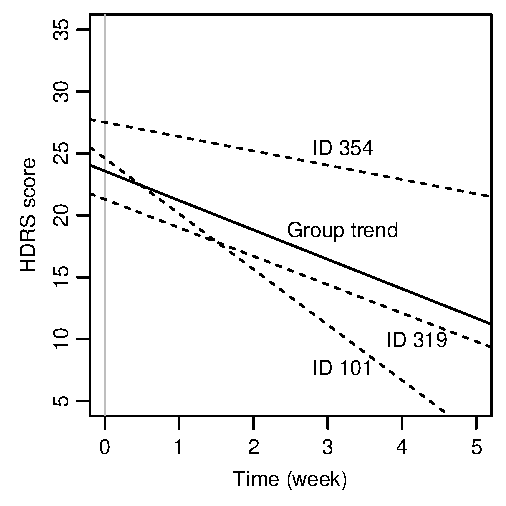
\includegraphics[width=5cm]{../figures/hdrs-lme2}
  \end{column}
  \begin{column}{.6\textwidth}
    \begin{itemize}
      \item The estimated mean baseline HDRS score is $\hat{\beta}_0 = 23.58$
      \item The estimated standard deviation between patients is
        $\hat{\sigma}_{\upsilon_0} = 3.55$
      \item The mean improvement per week is $\hat{\beta}_1 = -2.38$
      \item The estimated standard deviation between patients is
        $\hat{\sigma}_{\upsilon_1} = 1.44$
    \end{itemize}
  \end{column}
\end{columns}
  \begin{itemize}
    \item The estimated correlation between individual intercepts and
      slopes is $\hat{\varrho}_{\upsilon_0 \upsilon_1} = -0.28$
    \item Patients with higher (that means worse) baseline scores improve
      more strongly than patients with smaller baseline scores
  \end{itemize}
\end{frame}

\begin{frame}{Implied marginal covariance matrix}
  \begin{itemize}
    \item For the three time points $t_{ij} = 0, 1, 2$,
\[
  \mat{Z}_i =
    \begin{pmatrix}
      1 & 0 \\
      1 & 1 \\
      1 & 2 \\
    \end{pmatrix}
  \text{ und }
  \gmat{\Sigma}_\upsilon =
    \begin{pmatrix}
      \sigma^2_{\upsilon_0} & \sigma_{\upsilon_0 \upsilon_1} \\
      \sigma_{\upsilon_0 \upsilon_1} & \sigma^2_{\upsilon_1}
    \end{pmatrix}
\]
we get
\begin{align*}
  & Cov(\vect{y}_i) =
    \mat{Z}_i \gmat{\Sigma}_\upsilon \mat{Z}'_i + \sigma^2 \mat{I}_{n_i} \\
  &= \begin{pmatrix}
    \sigma^2_{\upsilon_0}                                    & \sigma^2_{\upsilon_0} + \sigma_{\upsilon_0 \upsilon_1}                             & \sigma^2_{\upsilon_0} + 2 \sigma_{\upsilon_0 \upsilon_1} \\
    \sigma^2_{\upsilon_0} + \sigma_{\upsilon_0 \upsilon_1}   & \sigma^2_{\upsilon_0} + 2 \sigma_{\upsilon_0 \upsilon_1} + \sigma^2_{\upsilon_1}   & \sigma^2_{\upsilon_0} + 3 \sigma_{\upsilon_0 \upsilon_1} + 2 \sigma^2_{\upsilon_1} \\
    \sigma^2_{\upsilon_0} + 2 \sigma_{\upsilon_0 \upsilon_1} & \sigma^2_{\upsilon_0} + 3 \sigma_{\upsilon_0 \upsilon_1} + 2 \sigma^2_{\upsilon_1} & \sigma^2_{\upsilon_0} + 4 \sigma_{\upsilon_0 \upsilon_1} + 4 \sigma^2_{\upsilon_1} \\
  \end{pmatrix}
   + \sigma^2 \mat{I}_{n_i}
\end{align*}
\item Hence, a more flexible covariance structure when compared to compound
  symmetry
  \end{itemize}
\end{frame}

\begin{frame}[fragile]{Fitting mixed-effects models}
\begin{lstlisting}
# random intercept model
lme1 <- lmer(hamd ~ week + (1 | id), dat, REML = FALSE)
summary(lme1)

# random slope model
lme2 <- lmer(hamd ~ week + (week | id), dat, REML = FALSE)
summary(lme2)

# model comparison
anova(lme1, lme2)
\end{lstlisting}
\end{frame}
 
\begin{frame}{Wald test}
  \begin{itemize}
    \item For the fixed effects, based on the covariance matrix
\[
  Var(\gvect{\hat\beta}) = \left( \sum_{i = 1}^N
    \mat{X}'_i \gmat{\Sigma}_i^{-1} \mat{X}_i \right)^{-1}
\]
we can construct Wald tests analogously to the regular linear model with
  approximately normally or $t$ distributed test statistics

    \item First, $\gmat{\Sigma}_i$ must be estimated; hence, the quality of the
      approximation strongly depends on the quality of the estimation of the
      variance and covariance components

    \item Many authors principally discourage using Wald tests for random
      effects \citep[e.\,g.,][p.~52 or \texttt{?lme4::pvalues}]{Hedeker2006}
  \end{itemize}
\end{frame}


\begin{frame}{Likelihood ratio test}
  \begin{itemize}
    \item Hypotheses about fixed and random effects can be tested with
      likelihood ratio tests
    \item When $M_0$ is a model that results from a more general model $M_1$ by
      parameter restrictions, then the test statistic
\[
  G^2 = 2\log \frac{L(M_1)}{L(M_0)}
      = 2\,(\log L(M_1) - \log L(M_0))
\]
  is approximately $\chi^2$ distributed with $(\text{Number of parameters
  in } M_1) - (\text{Number of parameters in } M_0)$ degrees of
  freedom
    \item However, for fixed effects this test can result in progressive test
      decisions for small samples (H$_0$ is rejected too often)
    \item For random effects and hypotheses of the form H$_0$:
      $\sigma^2_\upsilon = 0$, the test is rather conservative
  \end{itemize}
  \nocite{BrykRaudenbush2002}
\end{frame}
 
 
% \begin{frame}{Parametrisches Bootstrapping}
% Zur Absicherung der Ergebnisse des Likelihoodverhältnistests bietet sich ein
% parametrisches Bootstrapverfahren an:\\[2ex]
% 
% \begin{itemize}
% \item Anpassen des allgemeinen ($M_1$) und restringierten Modells ($M_0$) an
% die Daten. Berechnung der $G^2$-Statistik.
% 
% \item Simulation von $B$ Bootstrap-Stichproben $\vect{x}^{*B}$ auf Basis
% der stochastischen Komponente von $M_0$: Für diese Stichproben gilt H$_0$.
% 
% \item Für jede Bootstrap-Stichprobe: Anpassen von $M_1$ und $M_0$ und
% Berechnung einer Bootstrap-Replikation von $G^2$.
% 
% \item Bestimmung der Signifikanz von $G^2$ anhand der empirischen
% Stichprobenverteilung der Bootstrap-Replikationen.
% \end{itemize}
% \end{frame}
% 
% 
% \subsection{Modell mit zeitlich variierenden Kovariablen}
% 
% 
% \begin{frame}{Modell mit zeitlich variierenden Kovariablen}
% \begin{align*}
% \text{(Ebene 1)}  \quad y_{ij} &= b_{0i} + b_{1i}\,t_{ij} + b_{2i}\,x_{ij}
%                                   + \varepsilon_{ij}\\
% \text{(Ebene 2)}  \quad b_{0i} &= \beta_0 + \beta_3 \, g_i + \upsilon_{0i}\\
%                   \quad b_{1i} &= \beta_1 + \upsilon_{1i}\\
%                   \quad b_{2i} &= \beta_2\\
% \text{(2) in (1)} \quad y_{ij} &= \beta_0 + \beta_1\,t_{ij} +
%     \beta_2\,x_{ij} + \beta_3\,g_i + \upsilon_{0i} +
%     \upsilon_{1i}\, t_{ij}  + \varepsilon_{ij}
% \end{align*}
% Zeitlich variierende Kovariablen gehen als Ebene-1-Effekte in das Modell ein.
% Variablen, die über die Zeit konstant bleiben, dagegen als Ebene-2-Effekte, da
% sie nur zwischen Personen variieren.
% \end{frame}

\begin{frame}[<+->]{Summary}
  \begin{itemize}
    \item Assumptions of repeated measures ANOVA are often too restrictive
      for measurements taken over time
    \item Mixed-effects models allow for a more flexible variance-covariance
      structure
    \item For unequal group sizes, repeated measures ANOVA is not defined
    \item (For within designs where assumptions of equal variance are more
      plausible, repeated measures ANOVA is well suited)
  \end{itemize}
  \vfill
\end{frame}

\begin{frame}[fragile]{}
  \begin{block}{Exercise}
    \begin{itemize}
      \item Expand the linear mixed-effects model to more than one factor:
        \begin{itemize}
          \item Add diagnosis (``endogenous`` vs.\ ``non-endogenous'') as
            additional between factor
        \end{itemize}
      \item Test if this factor interacts with \texttt{week} using a
        likelihood-ratio test
      \item Use parametric bootstrapping to get a sampling distribution for your
        LRT statistic
      \item Plot the sampling distribution and add the empirical confidence
        interval
    \end{itemize}
  \end{block}
\end{frame}

\appendix

% \section{Expanding the model to more than one factor}
% 
% \begin{frame}{Two types of depression}
% \begin{center}
% 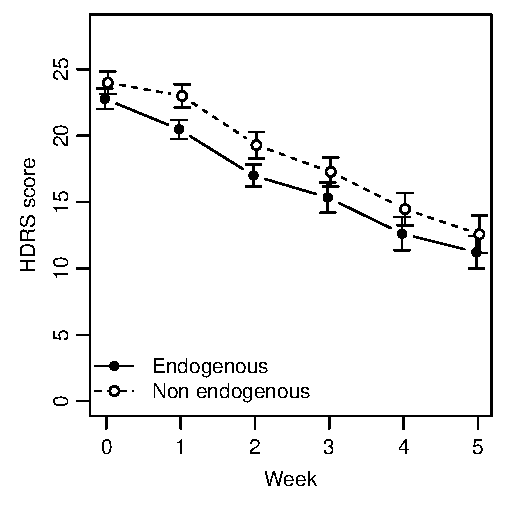
\includegraphics[scale=.8]{../figures/hdrs-means-se}
% \end{center}
% \end{frame}
% 
% \begin{frame}[fragile]{Fitting repeated-measures ANOVA}
%   \begin{lstlisting}
% # ANOVA with aov()
% aov2 <- aov(hamd ~ week2 * diag + Error(id/week2), dat_val)
% summary(aov2)
% 
% # Using ezANOVA()
% ez2 <- ezANOVA(data = dat_val, dv = hamd, wid = id,
%                within = week2, between = diag,
%                type = 1)
% ez2$ANOVA
%   \end{lstlisting}
% \end{frame}
% 
% \begin{frame}[fragile]{Fitting repeated-measures ANOVA}
%   \begin{lstlisting}
% # Mixed-effects model
% lme2 <- lmer(hamd ~ week2 * diag + (1 | id), dat_val)
% anova(lme2)
% 
% # Calculate mean sum of squares for id by hand
% sp <- attr(VarCorr(lme2)$id, "stddev")
% se <- attr(VarCorr(lme2), "sc")
% se^2 + 6 * sp^2
%   \end{lstlisting}
% \end{frame}
% 
% \begin{frame}[fragile]{Fitting mixed-effects model}
%   \begin{lstlisting}
% # And this works on the complete data set
% lme3 <- lmer(hamd ~ week2 * diag + (1 | id), dat)
% anova(lme3)
% 
% # Type I sum of squares
% lmerTest:::anova.lmerModLmerTest(lme3)
% 
% # Or via likelihood ratio tests
% m0 <- lmer(hamd ~ 1 + (1 | id), dat, REML=FALSE)
% m1 <- lmer(hamd ~ week2 + (1 | id), dat, REML=FALSE)
% m2 <- lmer(hamd ~ week2 + diag + (1 | id), dat, REML=FALSE)
% anova(m0, m1, m2, lme3)
%   \end{lstlisting}
% \end{frame}

%\begin{frame}[allowframebreaks]{References}
\begin{frame}{References}
  \printbibliography
  \vfill
\end{frame}

\end{document}

